\documentclass[UKenglish]{article}  %% ... or USenglish or norsk or nynorsk
\usepackage[utf8]{inputenc}           %% ... or latin1 or applemac
\usepackage[T1]{fontenc,url}
\urlstyle{sf}
\usepackage{tikz,babel,textcomp,csquotes,pgf-umlsd,varioref,graphicx}
\usetikzlibrary{arrows, shadows}
\title{Project 1}        %% ... or whatever
         %% ... if any
\author{Aulon Mujaj, Henning Lund-Hanssen, Espen Jones}                      %% ... or whoever 

\begin{document}
\maketitle{}

\section{Requirement 1 - Brief analysis}

\subsection{Brief description}
This program is a simulation of the popular game Minesweeper. In this version of
Minesweeper, the player is presented with a map of coordinates with
questionmarks. Under each questionmark, there is either a number representing
how many mines that are in the vicinity of this particular point on the map, or,
a mine. The player is prompted for a set of coordinates, which should correlate
to a questionmark on the map that the player does not think has a mine beneath
it. The game goes on for as long as the player does not hit a questionmark with
a mine beneath. The game ends when the player has identified all of the
questionmarks without a mine, or if the player hits a questionmark with a mine.
\subsection{Analysis}
\subsubsection{Defects}
This program consists of three files.

\begin{itemize}
    \item Minesweeper.java - The main class of this program. Calls on the two other parts, MineField and Ranking.
    \item MineField.java - Represents the map of the minefield
    \item Ranking.java - Handles the highscores of the players playing this game
\end{itemize}
\subsubsection{Minesweeper.java}
This main class on the program has the responsibility for the control flow of the program. When should the minefield be
called to make a judgement about whether the game is still going or ended? When should the ranking be upon to calculate
the score of the player and show the highscore? It taks input from the terminal and compares it to certain keywords. If
the input from the player does not match the input criteria, the game just prompts for new input.

The testable parts in this class consist of handling the input from the user and that the right action is taken
accordingly. For example, if the user gives "top" as input to the program, the ranking class should be called to show
the ranking of the players. And if restart is called, you would expect the program to restart your session.

\subsubsection{MineField.java}

\subsubsection{Ranking.java}

\subsection{Non-functional tests}
Non-functional tests should always be tested. Though, this code looks like it was submitted in some introduction course
in Java programming. If we look on this as a mandatory assignment in such a course, it should run on every machine at
UiO installed with Java. If this were to be a huge game developed by a real company with the goal of making a
multiplayer minesweeper with a regional highscore for each country and so on. The amount of non-functional requirements
will increase. 

We have decided to measure the non-functional requirements to meet what we can extract from the Minesweeper game on
Windows 10.

\subsubsection{Performance, load and stress}
The program should not strain the computer to the point where Minesweeper prevents normal execution of other programs. 

\subsubsection{Reliability}
If the program crashes, it does not save the state, so it is not recoverable after a crash. Though, the original game of
Minesweeper does not do this either.

\subsubsection{Usability}
Playing the game requires the player to have previous knowledge of coordination systems. The instructions on how to play
the game is lacking to some degree. It is a single line that instructs the user to give coordinates as input and to not
step on a mine. This is forgiving to some degree, as most of us have previous experience with the Minesweeper game.

\subsubsection{Efficiency}
The program operates instantaneously both when it comes to asking for input and calculating the highscore. Also, the
program as a whole does not utilize anything more than it needs to.

\subsubsection{Maintainability} % A bit functional??
If changes is to be made to this system, the programmer has to know the Java programming language. If not, it as to be
written from scratch in order for a change to be made. It is not imported or implemented a test library like JUnit for
testing the different parts of the program, so it is not easy to just implement new tests without interrupting the data
flow of the program.

\subsubsection{Portability}
The only requirement for the program to be run is Java. The program can be run automatically with an IDE like IntelliJ
or Eclipse. Without an IDE, you have to have some knowledge about the Java Platform. An alternative to just use the Java
compiler and platform is to use a software project management system like Maven, Ant or Make. They will shorten and ease
up the process of defining goals like compilation, testing and running the system standalone or for example with an
application server like Tomcat or Jetty


\subsection{Test cases}

\section{Requirement 2 - In-depth metrics}

\subsection{Metrics at project level}
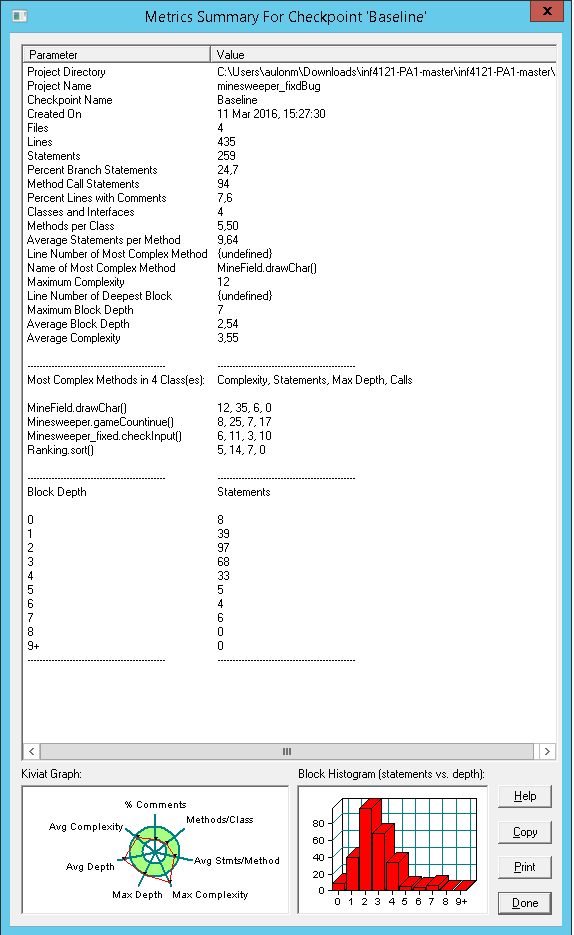
\includegraphics[height=8cm]{metric_summary}
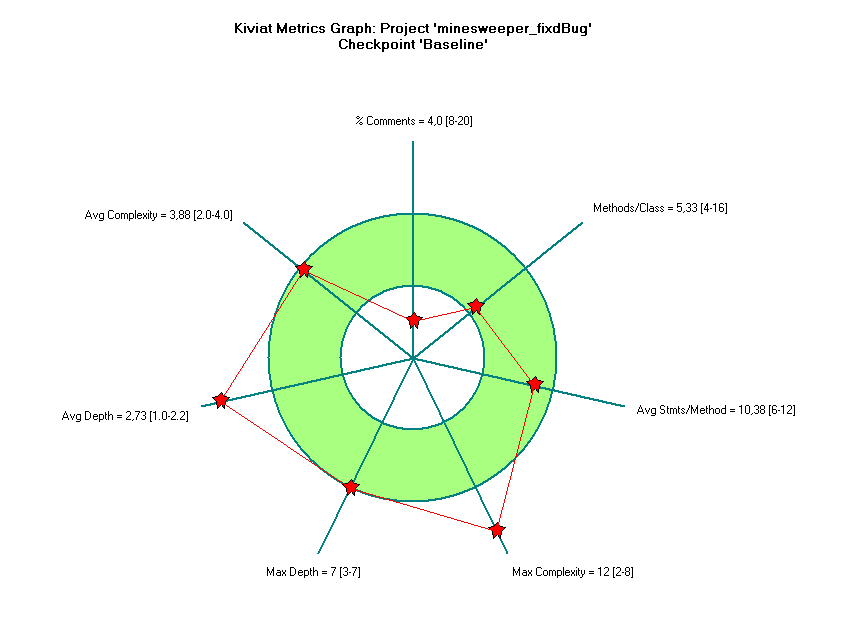
\includegraphics[height=8cm]{kiviat_diagram_baseline}
\begin{itemize}
\item What metrics do you spot for the whole project in the window Metrics Summary for Checkpoint? Write a brief description of the metrics. Try to explain their values (below what is expected, as expected or above the expected level). What metrics do you think need to change?\\
\item Which is the biggest file you have in your project by the number of lines of code? \\
MineField.java
\item Which is the file with most branches in your project?\\
\item Which is the file with most complex code? What metric did you choose to answer to this question?\\
Minesweeper.java
\end{itemize}

Write a little about each metric, maybe we'll only write about the 6 different metrics from the kiviat diagram, instead of each metric from the metric summary image?

If we choose to go only for the metrics from the kiviat diagram, then we'll only need to write about:\\
Avg complexity, avg depth, max depth, \% comments, methods/class, avg stats/method, max complexity\\\\
Files: This project that we are testing and analyzing has a total of three files\\\\
Lines: There are in total 326 lines of code throughout the three files. \\
Statements: Statements are terminated with a semicolon character in Java. Those lines of code are not the only ones that are statements, but branches suchs as if, for and while are also counted as statements. At the same time, exception control statemens try, catch and finally are also counted as statements, and throw statements. Our project that we chose has in total 162 statements. \\\\
Percent Branch statements: There are multiple statements that are regarded as branch statements. These are; if, else, for do, while, break, continue, switch, case and default, but we also count exception block statements such as try, catch, finally and throw as branch statements. The percent branch statements is how much percent of all the statements are branch statements in our project. This number in our project is 10.5\% which means that out of 162 statements, 16 of those are branch statements\\\\
Method call statements: All calls are counted, both in statements and in logical expressions. Our porject has 92 method call statements.\\\\
Percent lines with comments: Off all the lines throughout the three files, the percentage that are comments is 4\%. Which means that from 326 lines of code, 13 lines are comments. This isn't that much really, but if the code is easy to read and understand, that it does not really matter. If the code is unreadable with obscure variable names and complex logic, then it needs more comments. \\\\
Classes and Interfaces: SourceMonitor checks for the name ``class <class name>'' or ``interface <interface name>'' and extracts the class names. Both interfaces and classes are counted together. Our project has only three classes and no interfaces. \\\\ 
Methods per class: 
Average Statements per Method:
Name of Most complex methods
Maximum Complexity
Maximum Block Depth
Average Block Depth
Average Complexity
Most complext methods (complexity, statements, max depth, calls)
How many statements on each block depth



\subsection{Metrics at file level}
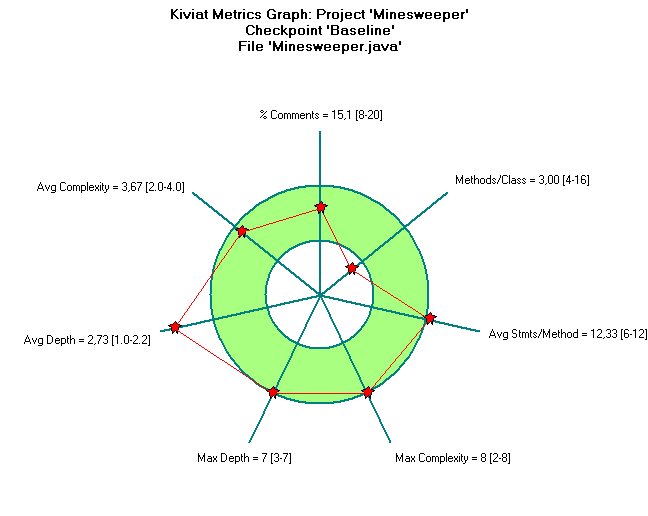
\includegraphics[height=8cm]{kiviat_diagram_minesweeper}
\begin{itemize}
\item How do you interpret the metrics applied on your file? How are they different the metrics you optained on the whole project, compared with the metrics ont his file?\\
\item Would you refactor (re-write) any of the methods you have in this file?
\end{itemize}
\section{Requirement 3 - Code improvement}

\subsection{Identification of metrics}

\subsection{Results from changes}

\subsection{Final remarks}

\end{document}
